\documentclass{article}
\usepackage{enumitem}
\usepackage{listings}
\usepackage{amsfonts}
\usepackage{latexsym}
\usepackage{fullpage}
\usepackage{graphicx}
\usepackage{paralist}
\usepackage{tikz-timing}

\lstdefinelanguage{VHDL}{
  morekeywords={
    library,use,all,ENTITY,IS,PORT,IN,OUT,end,architecture,of,
    begin,and, ARCHITECTURE, IF, THEN, SIGNAL,END, PROCESS
  },
  morecomment=[l]--
}

\usepackage{xcolor}
\colorlet{keyword}{blue!100!black!80}
\colorlet{comment}{green!90!black!90}
\lstdefinestyle{vhdl}{
  language     = VHDL,
  basicstyle   = \ttfamily\scriptsize,
  keywordstyle = \color{keyword}\bfseries\ttfamily,
  commentstyle = \color{comment}\ttfamily,	
  tabsize=1
}

\renewcommand{\lstlistingname}{Code}

% Default margins are too wide all the way around. I reset them here
\setlength{\topmargin}{-.5in}
\setlength{\textheight}{9in}
\setlength{\oddsidemargin}{.125in}
\setlength{\textwidth}{6.25in}


%\let\oldenumerate\enumerate
%\renewcommand{\enumerate}{
  %\oldenumerate
  %\setlength{\itemsep}{1pt}
  %\setlength{\parskip}{0pt}
  %\setlength{\parsep}{0pt}
%}


\begin{document}
\title{Organization of Digital Computer Lab \\ EECS112L/CSE 132L}
\author{\textbf{Assignment 3 }\\ \textbf{Single-cycle MIPS - Complete} \\ \\
prepared by: Team Stressed \\ Student name: \\ Mansi Tyagi \\ Student ID: \\23334840\\ \\ Student name: \\ Erik Henriquez\\ Student ID: \\57374677\\ \\ Student name: \\ Kevin Chau \\ Student ID: \\76934313\\ \\ Student name: \\ Steven Chow\\Student ID: \\70916812\\ \\ Student name: \\ Paul Dao \\Student ID: \\30658761\\ \\
EECS Department\\ Henry Samueli School of Engineering \\ University of California, Irvine \\ \\
{February 21, 2016}} 


\date{}
\maketitle


\section{Summary of Processor Design}
\subsection{What We Learned}
After implementing a subset of MIPS R-type and I-type instructions in Lab 2, we implemented additional I-type instructions and added support for J-type instructions. After reviewing material we had previously learned in CSE 132, we were able to implement a complete single-cycle processor that met this assignment's specifications. For the synthesis portion of this assignment, we learned to use Synopsis for elaboration and to determine the power consumption, area requirements, and clock frequency necessary to build our processor design. Although the use of Synopsis was initially very troublesome, we appreciated the fact that we were able to use tools that well-known corporations, like Intel and AMD, use to design and fabricate their own products.

\subsection{Description}
For our complete single-cycle processor, we designed ten components: a Program Counter (PC), Controller, Instruction Memory (two versions), Register File, Arithmetic Logic Unit (including a Comparator), Data Memory (RAM), Adders, and the Processor entity. While most of these components existed in our previous processor design, they were all improved and/or modified to work with our new datapath design. The PC no longer increments an initialized variable every clock cycle; instead, it takes in an inputted address and outputs it every clock cycle, basically acting as a register. Our controller has a Branch port (that is being used) and a new Jump port, to enable the use of Branch and J-type instructions, respectively. During simulation, we use the same instruction memory (ROM) component, but we also wrote a ROM for synthesis that has instructions preloaded into its memory array. We changed the design of our Register File so it no longer used WAIT statements, which cannot be synthesized. Our ALU is roughly the same as before, with the exception of the missing Jump port that was moved to the Controller. Our Data Memory was also modified for synthesis, although we chose to use Professor Yaghini's SRAM component for our synthesis results. We created an Adder component to use for our Branch/Jump datapath. Finally, we updated the design of the Processor entity to include all our components and used combinational logic to mimic the multiplexors and logic gates needed along the datapath. 

The processor now supports the following branch and J-type instructions: beq, bne, bltz, bgez, blez, bgtz, jump, jr, jal and jalr. To support these instructions, we created a separate Branch/Jump datapath. Composed of two Adder components and combinational logic that acts as the required Shifters and Multiplexors, the new datapath runs alongside our old one. For branch instructions, the Controller and ALU must send branch signals before the PC can be changed appropriately. To do this, the Controller must recognize the instruction as a Branch instruction from the OpCode and the ALU must check if the branch condition (register equivalency, register difference, etc.) is met. For J-type instructions, only the Controller's Jump signal is needed to allow the modification to the PC.

\subsection{Testbench Architecture}
For the most part, our testbench is the same as the one that we used for our Lab 2 assignment. We added more cycles to accommodate for the additional instructions in our Instruction Memory. For example, we run two beq instructions (one fails and the other succeeds) and a jump instruction that goes into uninitialized memory.


\section{Sample Program}
\subsection{Instructions}
We were given a list of 18 32-bit MIPS instructions, written in hexadecimal form. Before proceeding, we decoded these instructions into a human-readable format.

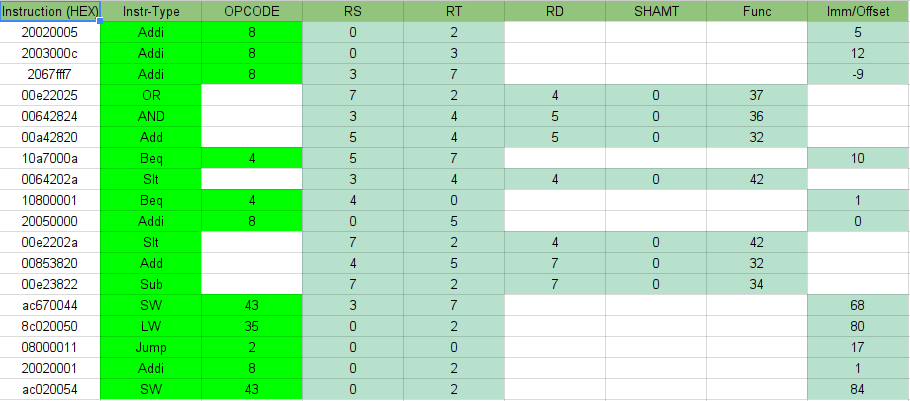
\includegraphics[width=0.8\textwidth]{example_program_decoded_instructions.png}

After decoding the instructions, we worked out the theoretical state of the Register File after every instruction. Of the two branch instructions in our sample program, one is successful and results in four instructions being skipped. There is also a jump instruction near the end of the program, which skips the final two instructions and moves the program counter into undefined memory, resulting in a "garbage" instruction. \\


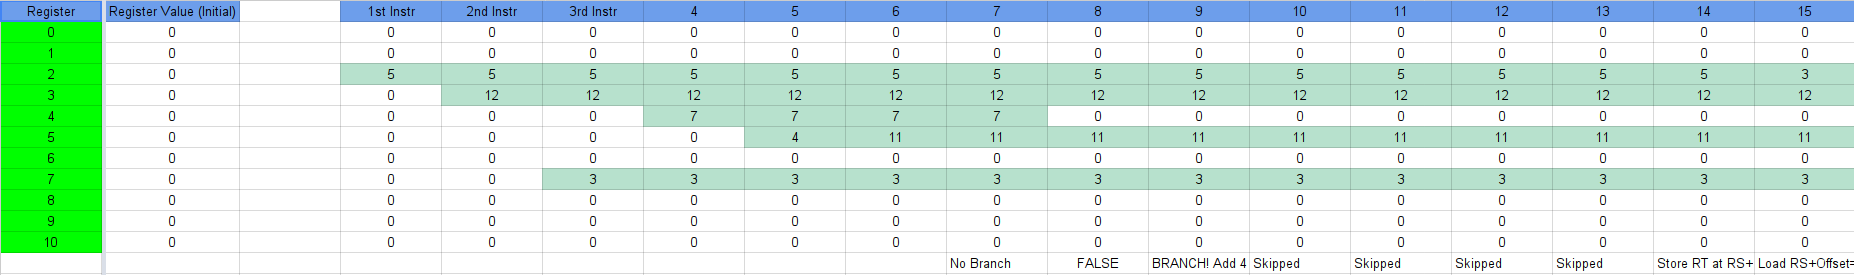
\includegraphics[width=0.8\textwidth]{example_program_registerfile_part1.png} \\ \\
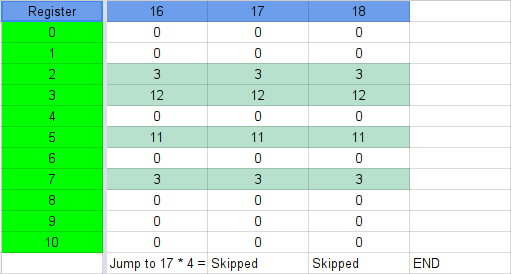
\includegraphics[width=0.25\textwidth]{example_program_registerfile_part2.png} 
	
\subsection{Simulation Waveform}
\bfseries{After designing and testing our Processor, we generated the following waveforms:} \\ \\
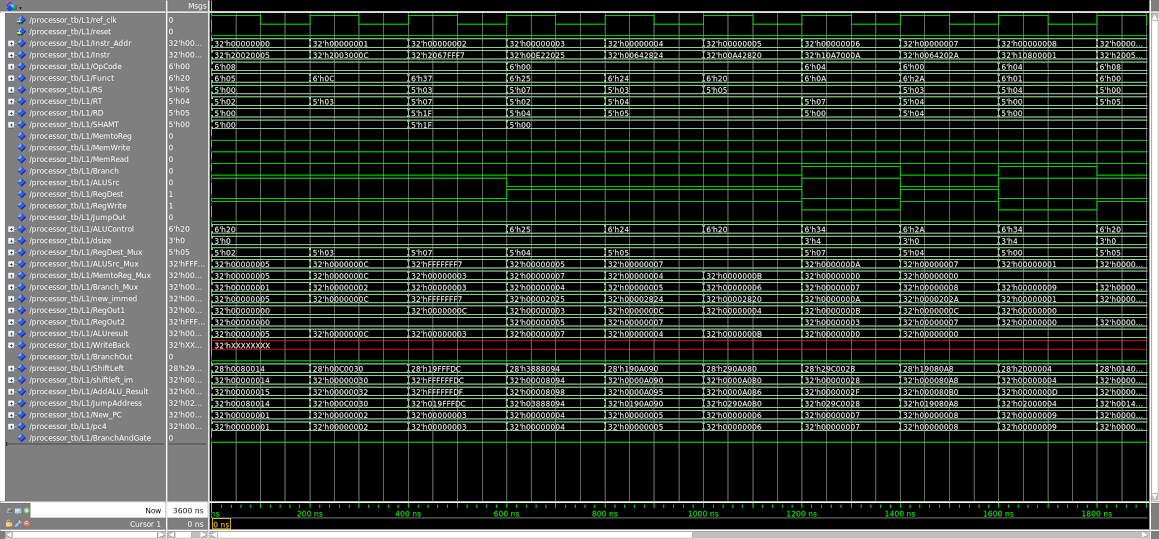
\includegraphics[width=0.8\textwidth]{waveform_part1.png} \\ \\
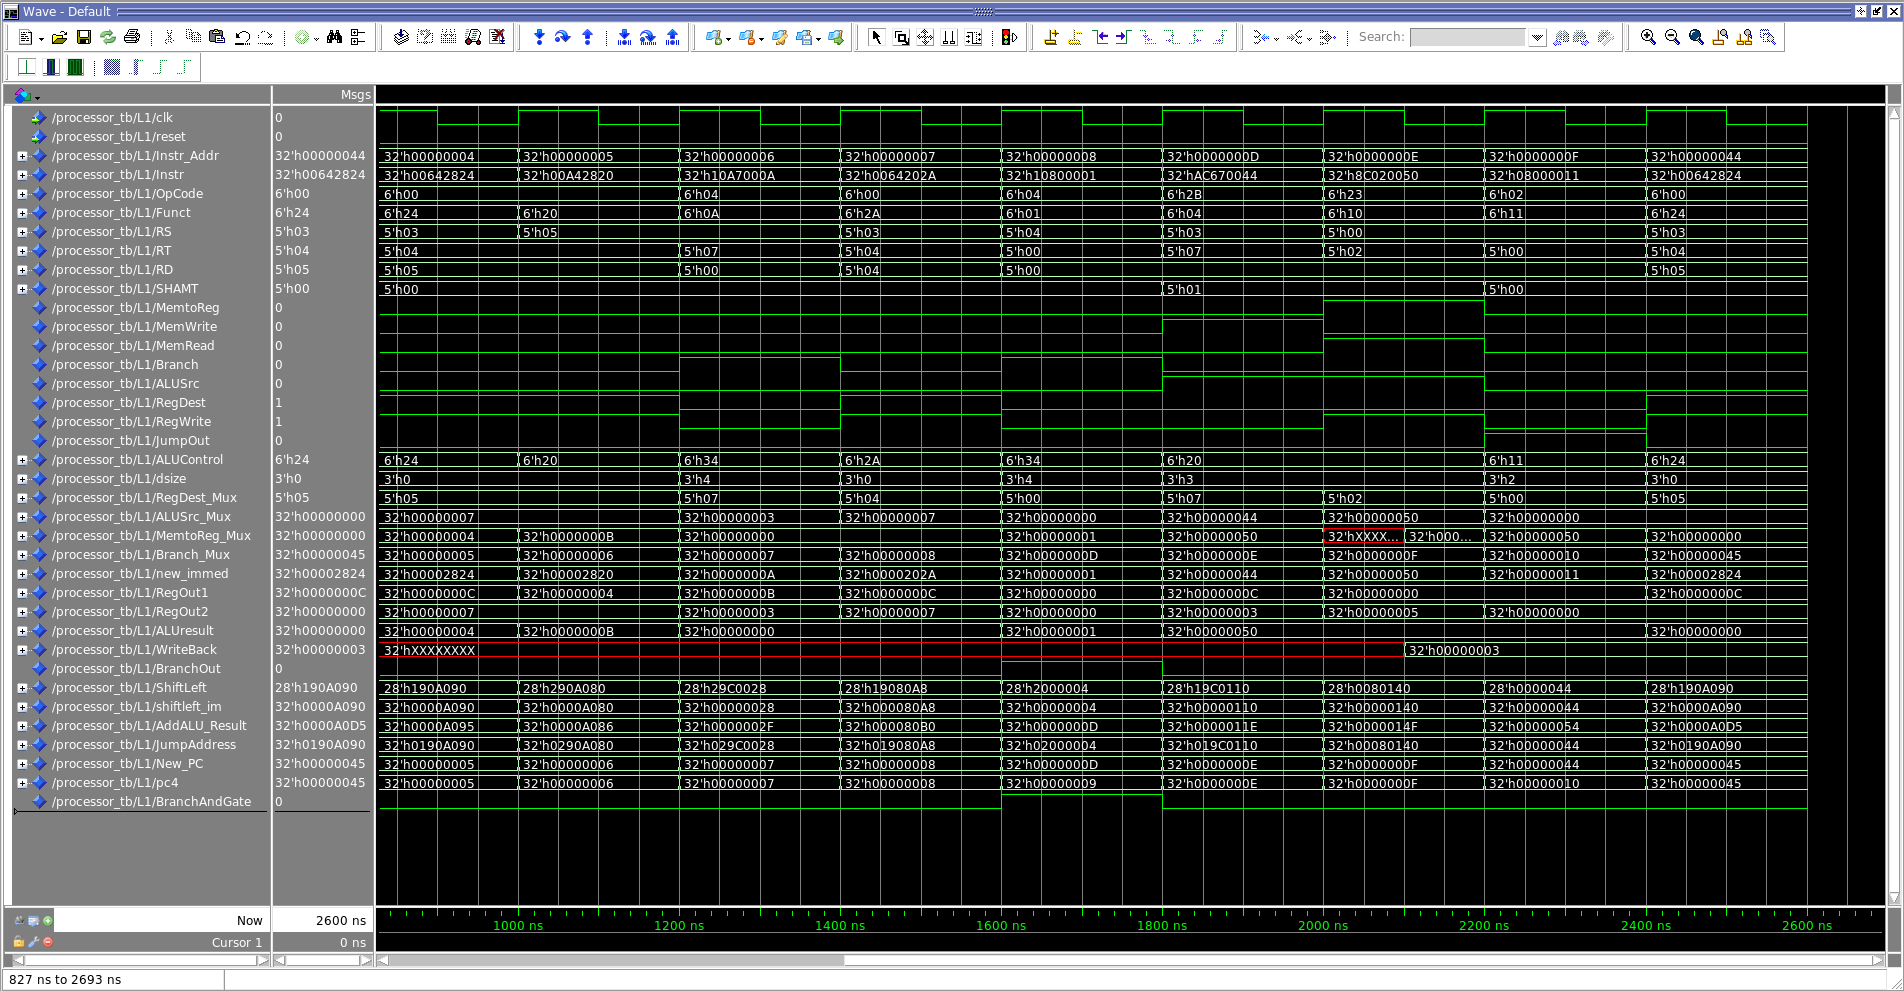
\includegraphics[width=0.8\textwidth]{waveform_part2.png} \\

As you can see, our branch and jump instructions worked as expected. Of the 18 instruction in the example program, only 12 were actually executed. We included a 13th cycle in our waveform to display the "garbage" instruction after our jump instruction.

\section{Synthesis}
Through synthesis, we were able to determine the power consumption, area requirements, and frequency of our processor design. Synopsis, a software suite provided by our university, was used to perform synthesis on our design. After adjusting the analysis, elaboration, and synthesis files and scripts, we synthesized our processor design and successfully generated various reports on our processor's performance.

\subsection{Power Consumption}
Our processor's total power consumption came out to 20.3 mW. From the power hierarchy we generated, approximately 74\% of the power consumption is due to our register file component, with another 19.9\% being used by the ALU. All other components use three orders of magnitude less power.

\subsection{Area}
After reading the generated area reports, we could not determine the units being used in the report. However, Synopsys reported that our Design area would be 82228.100300, with a Combinational Area of approximately 16868. We achieved these results using Professor Yaghini's SRAM. However, when using our Data Memory component (written in VHDL), our Combinational Area was over twice as large.

\subsection{Required Frequency}
According to the generated timing report, our Critical Path Length was 3.18 ns. In order to accommodate this and eliminate negative slack, we raised our clock period from 2.0 ns to 3.2 ns. This results in a frequency of approximately 312.5 MHz.

The majority of our timing delay comes from our PC adder, accounting for approximately 2.25 ns of the critical path length. We expect to see a reduction in the critical path in future labs, where our Adder components will not be required.

\section{Known Issues} 
Due to our unfamiliarity with SystemVerilog, we chose not to use the testbench to preload instruction memory. For the Questasim simulation, we read the example program instructions from a file.  For synthesis, we created a second version of instruction memory that has instructions preloaded into memory in order to synthesize the Processor properly.
\\
\section{Conclusion}

As a complete single-cycle processor, our project now supports a larger subset of the full MIPS instruction set. It is capable of all three types of MIPS instructions: R-type, I-type, and J-type. Through synthesis, we were able to determine the area, power and frequency properties our processor design would have if fabricated. Finally, with this complete processor, we should be well prepared to implement pipelining in our future assignment.


\end{document}
